\section{Data Sources and Construction}

\subsection{Trade values and quantities}

We construct monthly U.S. imports from the U.S. Census Bureau fixed-width merchandise-trade archives. The unit of observation is partner country $c$, ten-digit Harmonized System product $i$, and month $t$. The source fields are general customs value, general CIF value, first quantity, ordinary duty value, and calculated duty value. Each archive is parsed independently, aggregated to the canonical key, reconciled to its source total, and stored as ZSTD-compressed Parquet with source fingerprints.

Let $CIF_{ict}$ denote general CIF value, $Q_{ict}$ first quantity, and $D_{ict}$ calculated duties. The four import outcomes are
\begin{align}
m\_val_{ict}&=CIF_{ict}/10^6,&
m\_q1_{ict}&=Q_{ict}/10^6,\\
m\_p_{ict}&=CIF_{ict}/Q_{ict},&
m\_pduty_{ict}&=(CIF_{ict}+D_{ict})/Q_{ict}.
\end{align}
Unit values are defined only for positive quantities. Missing quantities and observed zeros are retained as distinct source states. In particular, duty-inclusive unit value uses observed Census calculated duties; it is not constructed by multiplying price by the independently reconstructed tariff.

\subsection{Tariffs}

The independently reconstructed bilateral tariff combines the applicable most-favored-nation rate with the trade-war increments:
\begin{equation}
\tau_{ict}=\tau^{MFN}_{it}+\Delta\tau^{201}_{ict}+\Delta\tau^{232}_{ict}+\Delta\tau^{301}_{ict}.
\end{equation}
The baseline and product schedules are taken from official USITC HTS releases, presidential proclamations, Federal Register annexes, and USTR Section 301 notices. Structured tables are used when available; reviewed PDF-table extractions are used for official annexes without a suitable tabular release. Each component retains its source, rate, legal date, and product/partner scope.

Consistent with the original paper's appendix, the construction excludes antidumping and countervailing duties, unrelated treaty changes, and quota-contingent increments that apply only once an entry-level threshold is crossed. Monthly partner--HS10 data do not identify the tier used by an individual customs entry. The original authors report that the affected quota-threshold varieties account for approximately \$16 million out of roughly \$300 billion in annual targeted imports.

\subsection{Timing conventions}

If an increment $\Delta\tau$ takes effect on day $d$ of a $D$-day month, the locked day-weighted initial-month increment follows days in effect:
\begin{equation}
\Delta\tau^{dw}_{t}=\Delta\tau\frac{D-d}{D},\qquad
\Delta\tau^{remainder}_{t+1}=\Delta\tau\frac{d}{D}.
\end{equation}
The paper-compatible event clock assigns the legal month when $d\leq15$ and the following month when $d>15$. The legal clock instead uses the calendar month containing the effective date. Only the paper-clock reconstruction is compared to the paper; the legal-clock curve is an alternative timing exercise.

Untreated products require an event origin to remain in the event-study controls. Following the Stata program, the date is assigned from the earliest date in the same NAICS4 industry, then NAICS3, then NAICS2. February 2018 is the final fallback. This operation does not change treatment status.

\section{Replication and Extension Results}

\subsection{Event-study specification}

The locked event study estimates
\begin{equation}
100\log y_{ict}=\sum_{k=-5}^{6}\beta_k\mathbf{1}\{T_i=1,event_{it}=k\}
+\sum_{k=-5}^{6}\gamma_k\mathbf{1}\{event_{it}=k\}
+\alpha_{ic}+\delta_{ct}+\eta_{it}+\varepsilon_{ict},
\end{equation}
where month $-6$ is omitted and the right tail is top-coded at $6+$. The fixed effects are product--country, country--month, and product--month. Standard errors are clustered by HS8 and partner country.

\begin{figure}[ht]
\centering
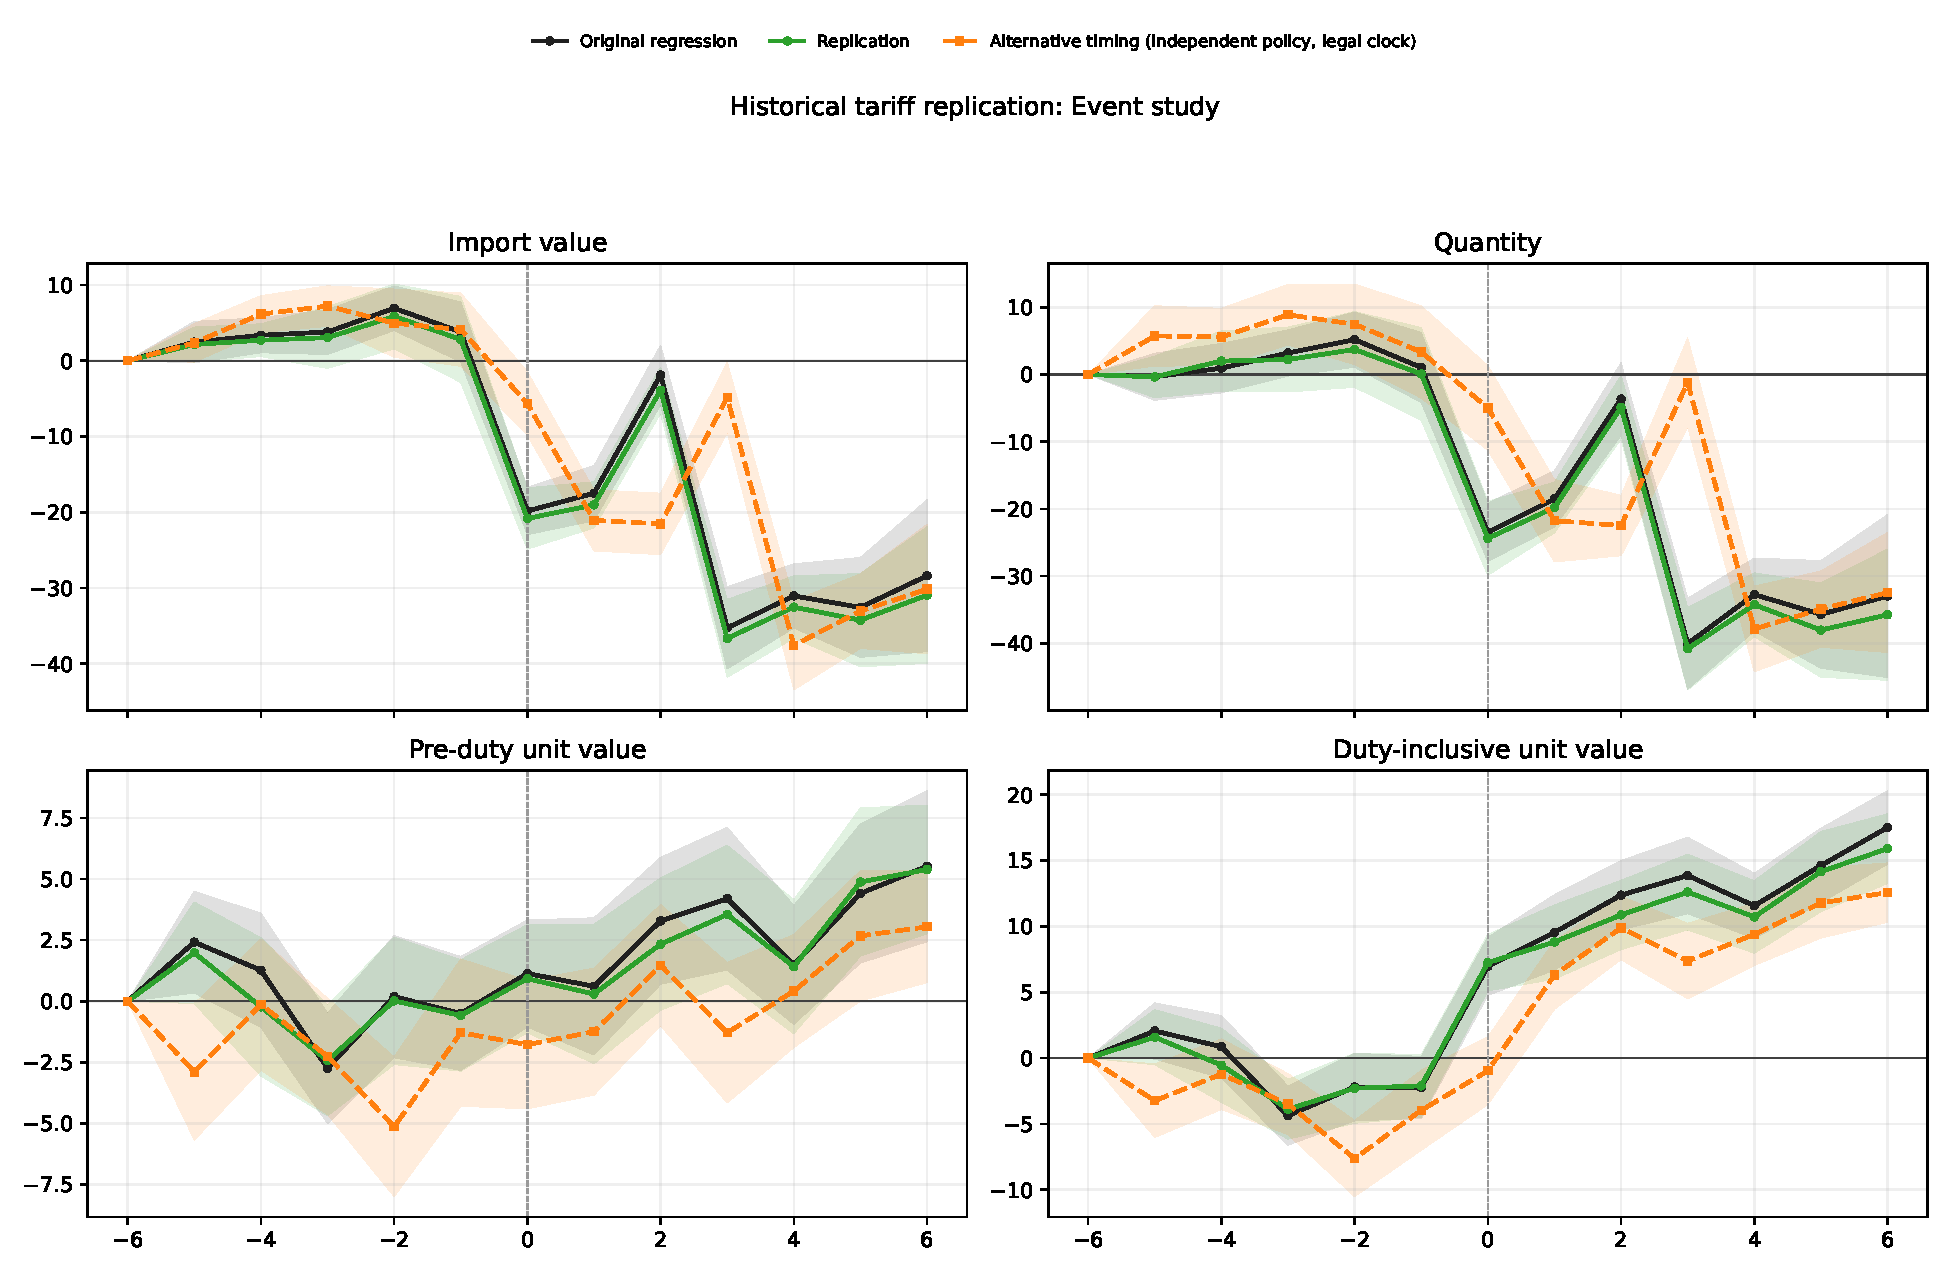
\includegraphics[width=0.96\textwidth]{../../figs/replication/historical_replication_event.pdf}
\caption{Locked historical event-study replication, $[-6,+6]$.}
\end{figure}

\subsection{Dynamic specification}

Let $x_{ict}=\Delta\log(1+\tau_{ict})$ and let $\Delta\ell y_{ict}$ be the first difference of the corresponding log outcome. We estimate
\begin{equation}
\Delta\ell y_{ict}=\sum_{k=1}^{6}\phi_{-k}F^kx_{ict}+\phi_0x_{ict}
+\sum_{k=1}^{K}\phi_kL^kx_{ict}+\eta_{it}+\delta_{ct}+\kappa_{cs}+u_{ict},
\end{equation}
including the missing-lead and missing-lag indicators used by the original
Stata code. Fixed effects are product--month, country--month, and
country--NAICS4; clustering is by HS8 and country. Plotted effects are
cumulative linear combinations, with standard errors computed from the full
covariance matrix. The paper replication sets $K=6$. Appendix Figure~2 plots
the independent reconstruction through $K=12$, while the separately labeled
long-horizon exercise sets $K=24$; neither changes the locked authors-package
benchmark.

\begin{figure}[ht]
\centering
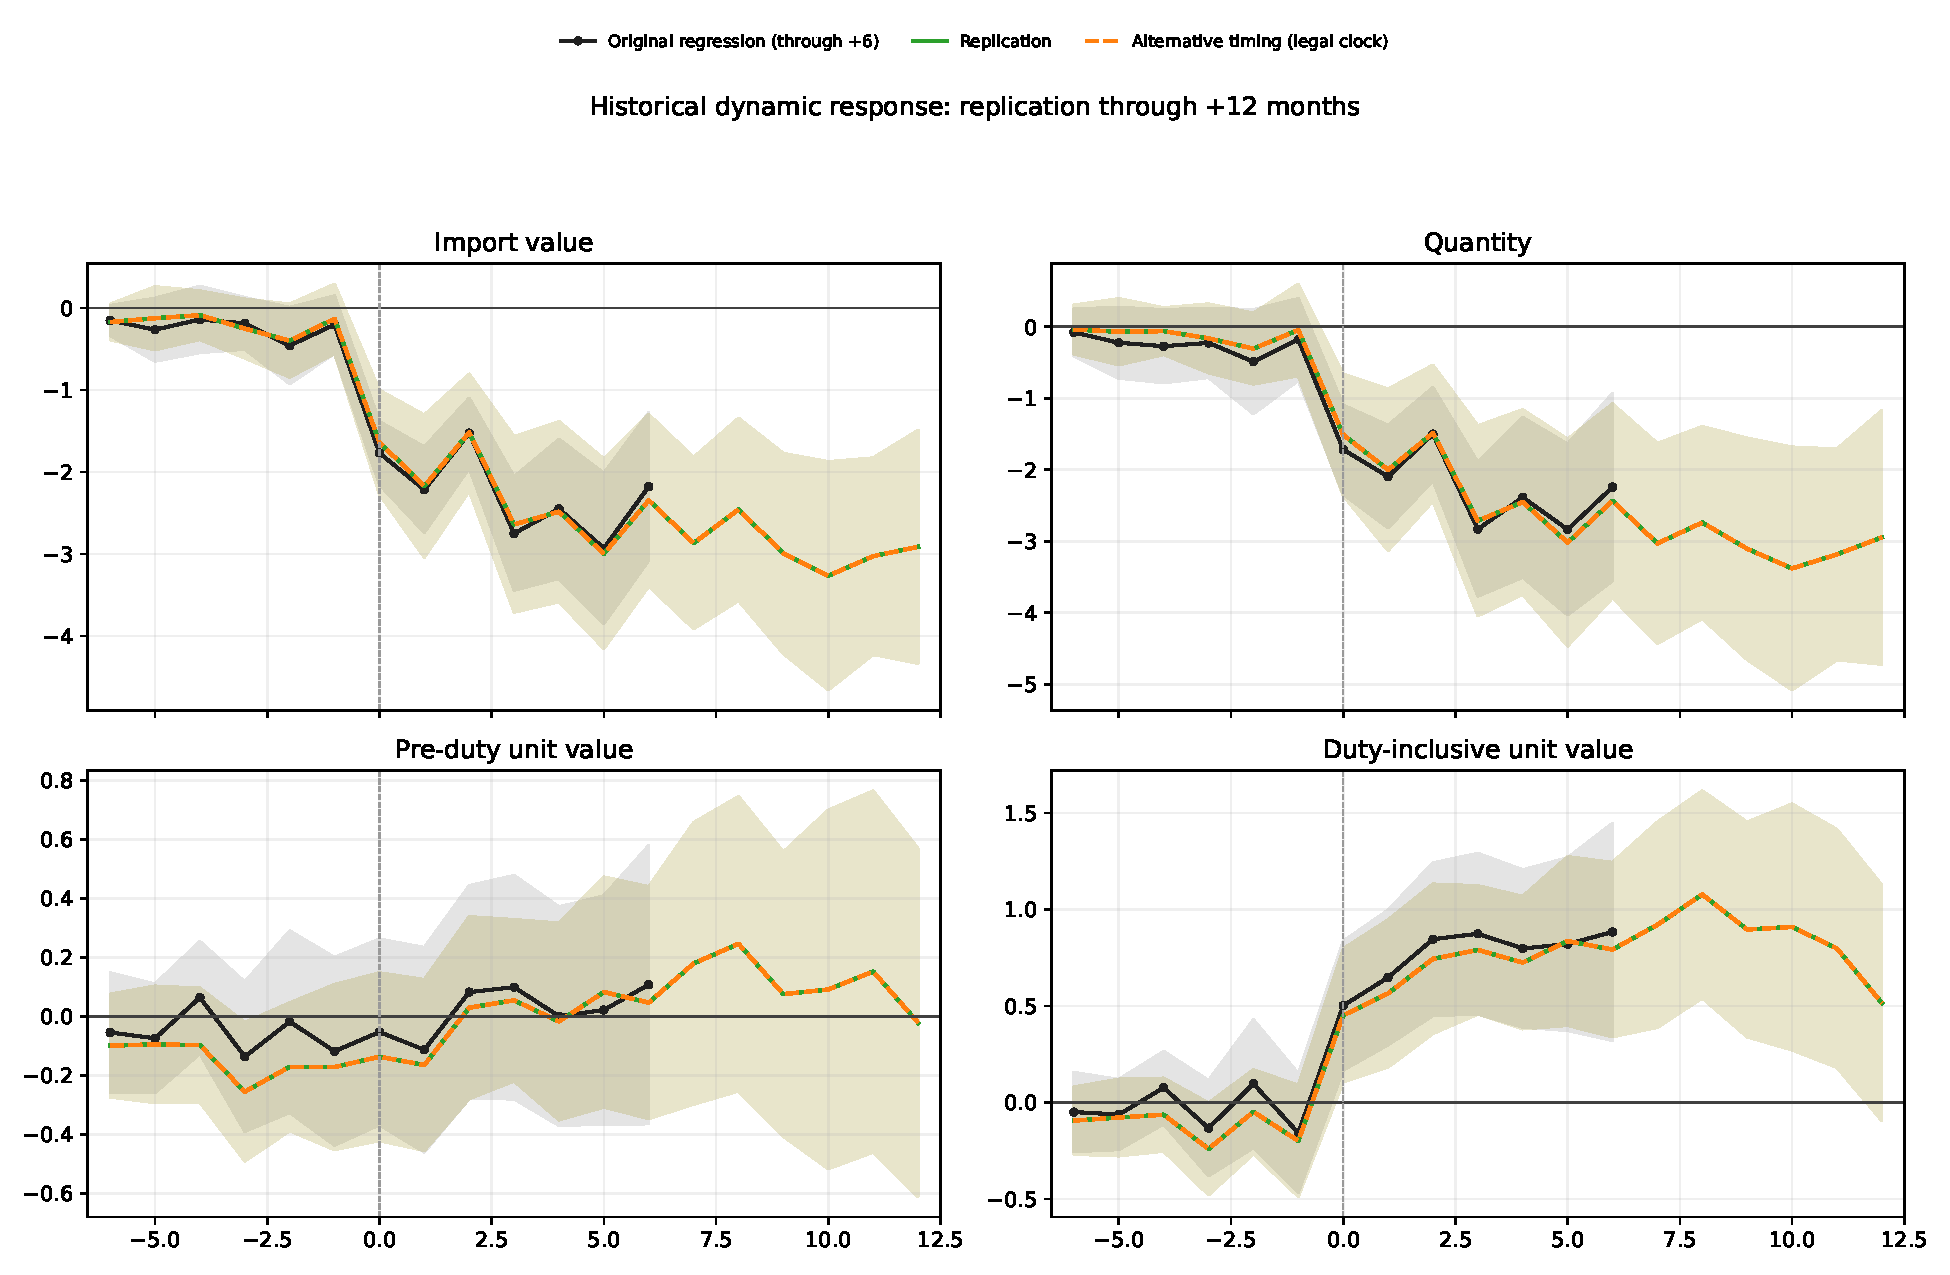
\includegraphics[width=0.96\textwidth]{../../figs/replication/historical_replication_dynamic_h12.pdf}
\caption{Historical dynamic pass-through. The original-regression benchmark
remains locked at $[-6,+6]$; the independent replication and legal-clock
sensitivity continue through $+12$ using the validated longer-horizon
coefficients.}
\end{figure}

\subsection{Validation evidence}

The package-only Python estimator produces eight import fits with thirteen horizons each. Across 104 PDF reference points, the maximum absolute difference is 1.009620 log points, below the preregistered 1.10 tolerance.

Table~\ref{tab:policy} compares the independently reconstructed paper-clock policy with the authors' policy anchor while holding the raw Census outcome sample fixed. Seven of eight point-estimate comparisons satisfy the registered thresholds. Event-study quantity is the disclosed exception.

\begin{table}[ht]
\centering
\caption{Independent policy substitution on the common raw-outcome sample}
\label{tab:policy}
\begin{tabular}{llrrr}
\toprule
Specification & Outcome & Correlation & RMSE & Maximum difference\\
\midrule
Event & Value & 0.9994 & 1.0727 & 1.9403\\
Event & Quantity & 0.9984 & 1.5650 & 2.6478\\
Event & Pre-duty price & 0.9703 & 0.5280 & 1.4191\\
Event & Duty-inclusive price & 0.9979 & 0.4691 & 1.4172\\
Dynamic & Value & 0.9986 & 0.1203 & 0.2338\\
Dynamic & Quantity & 0.9970 & 0.1663 & 0.2989\\
Dynamic & Pre-duty price & 0.9599 & 0.0307 & 0.0595\\
Dynamic & Duty-inclusive price & 0.9978 & 0.0404 & 0.0891\\
\bottomrule
\end{tabular}
\end{table}

The accepted decision is therefore \emph{historical methodology accepted with a disclosed quantity exception}. It is not an assertion that the formal eight-of-eight policy gate passed. The corresponding figures distinguish the original package regression, the independent paper-clock replication, and the independent legal-clock alternative.

\subsection{Longer horizon}

The separate $[-6,24]$ exercise uses archive-native CIF trade through October 2020. The original package series remains locked to $[-6,6]$. Because post-April-2019 actions are outside the validated historical tariff ledger, the extension freezes the April 2019 bilateral tariff level. It is therefore a persistence exercise under the locked historical treatment, not an estimate of later tariff actions and not a 2025 event study.

\begin{figure}[ht]
\centering
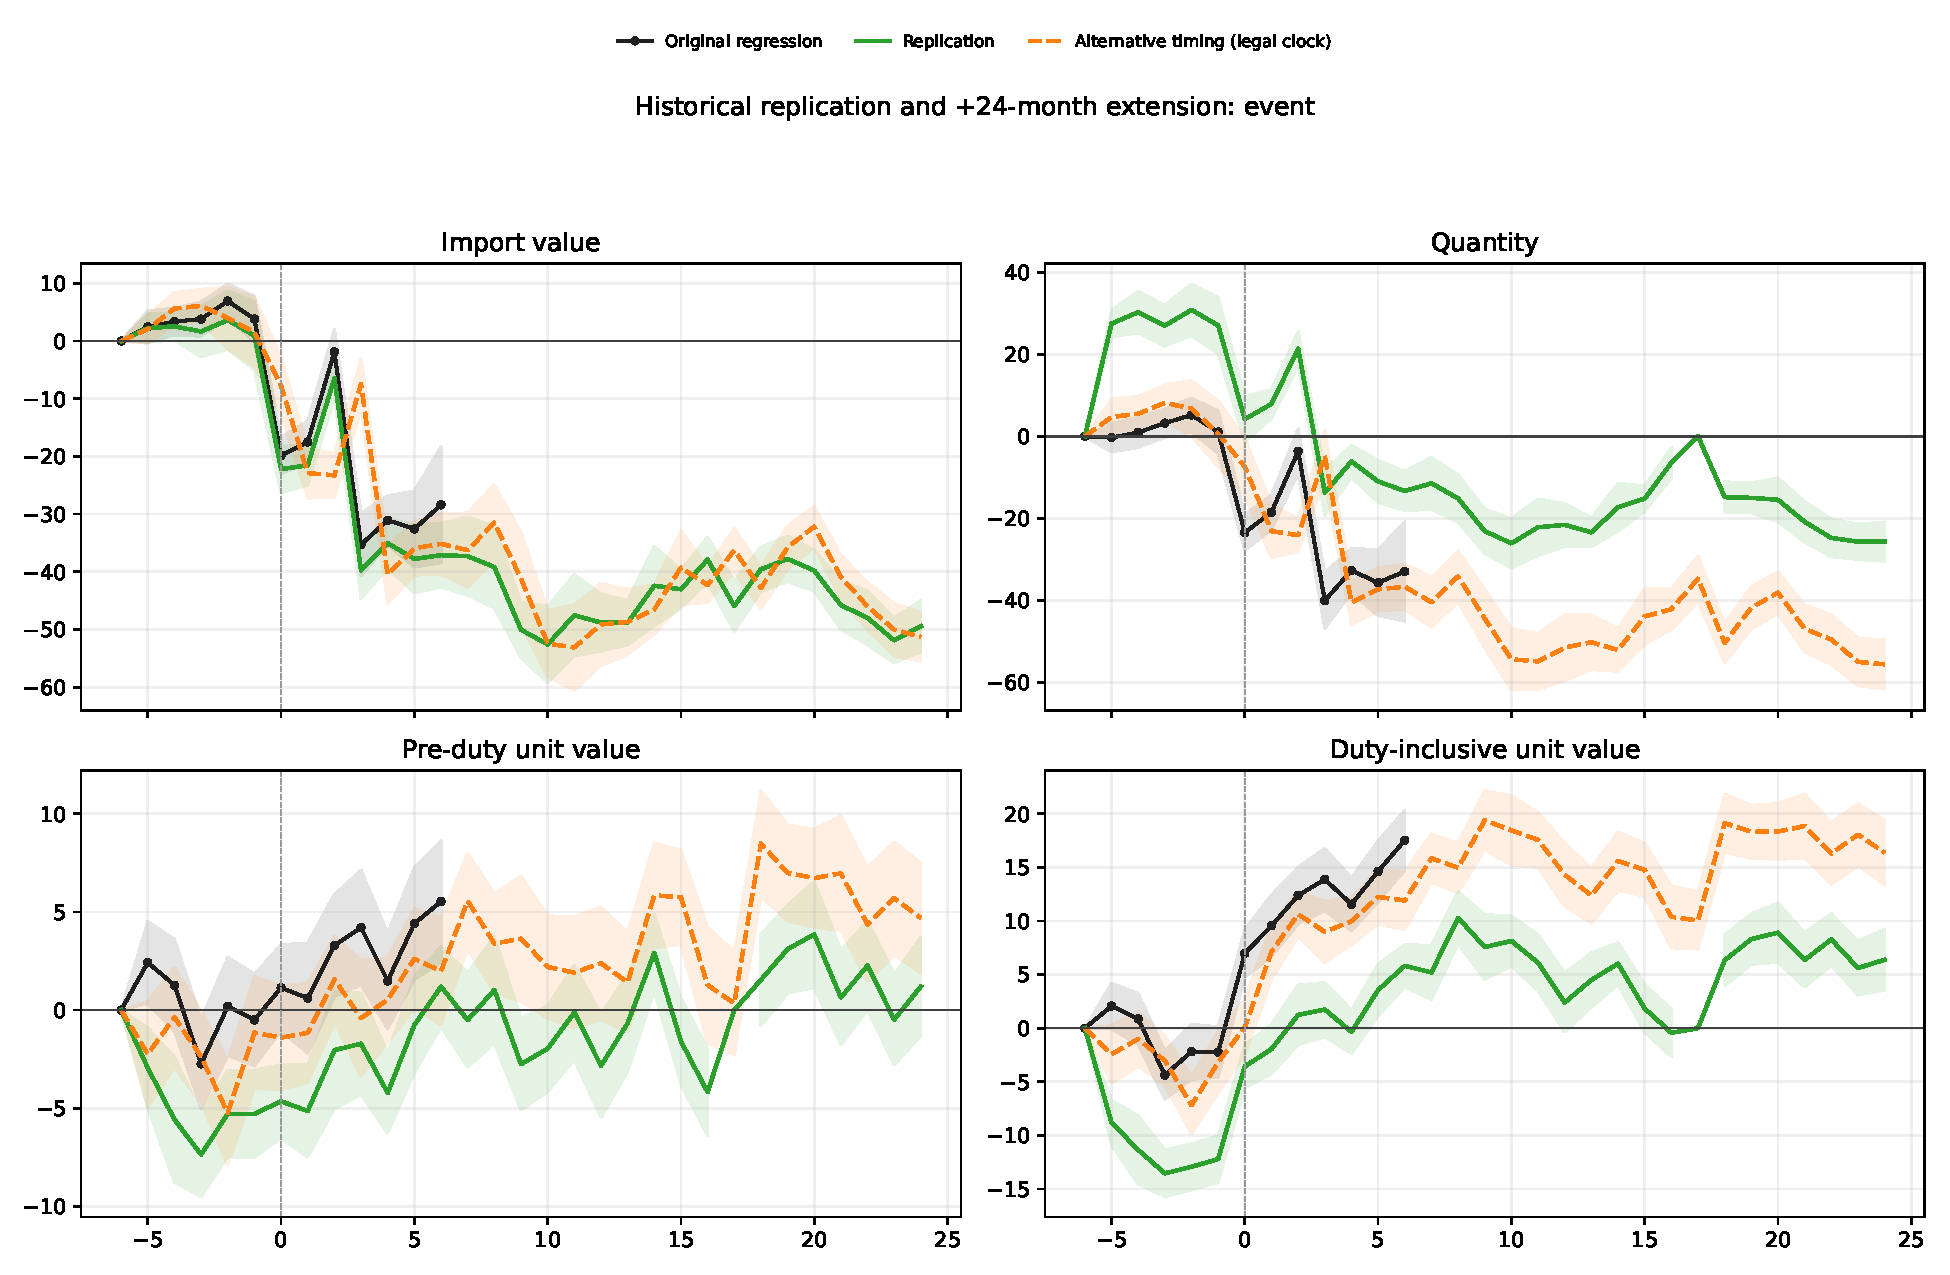
\includegraphics[width=0.96\textwidth]{../../figs/replication/historical_replication_event_h24.pdf}
\caption{Historical event-study persistence exercise, $[-6,+24]$.}
\end{figure}

\begin{figure}[ht]
\centering
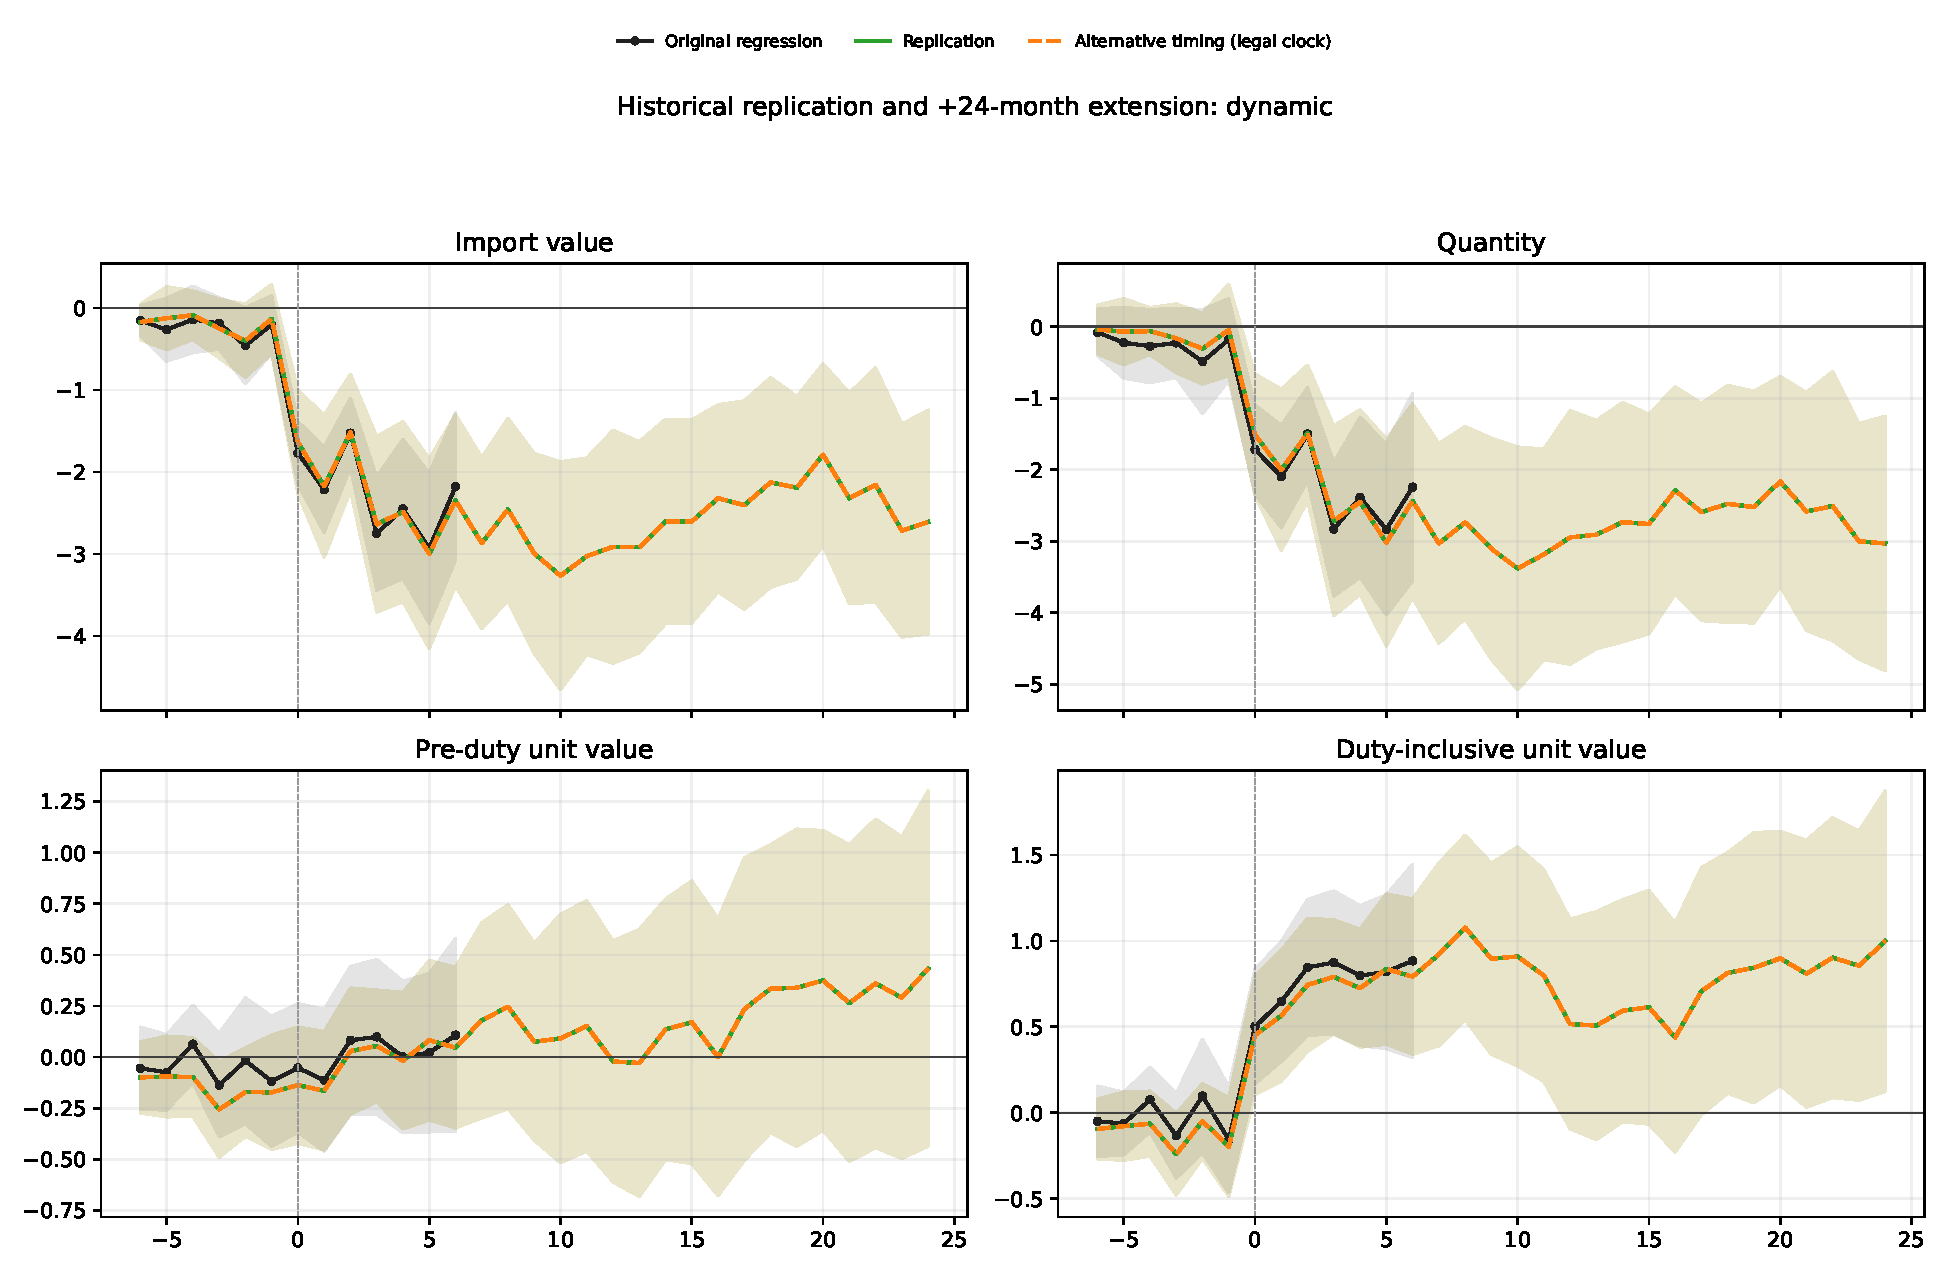
\includegraphics[width=0.96\textwidth]{../../figs/replication/historical_replication_dynamic_h24.pdf}
\caption{Historical dynamic persistence exercise, $[-6,+24]$.}
\end{figure}

\section{The 2025 Tariff Episode under the Fajgelbaum--Khandelwal Design}

\subsection{Applied-tariff data}

For the 2025 application we follow Fajgelbaum and Khandelwal (2026) rather
than imposing a common statutory event date.  The Census import-detail files
report imports for consumption separately by origin, ten-digit HTS product,
month, and rate provision.  We first aggregate districts and sub-country
records within rate provision, and then aggregate the fifteen provisions to
the origin--product--month variety.

Let $V_{igt}$ be consumption customs value, $Q_{igt}$ first consumption
quantity, and $D_{igt}$ recorded calculated duty.  The realized tariff and
unit values are
\begin{align}
\tau^{applied}_{igt}&=D_{igt}/V_{igt},\\
p_{igt}&=V_{igt}/Q_{igt},&
p^{duty}_{igt}&=(V_{igt}+D_{igt})/Q_{igt}.
\end{align}
These definitions replace the superseded construction that combined
general-import CIF and quantity with consumption duties.  Rate provision 79
contains Chapter 99 imports for which Census does not report calculated
duties.  We do not impute an unobserved duty. The canonical measure retains
provision-79 value in the denominator, sums only recorded duties, and flags the
resulting applied rate as incomplete. A separately labeled sensitivity excludes
provision 79 from both numerator and denominator.

\subsection{Local-projection event study}

For each variety, treatment begins in the first month in which the applied
tariff exceeds its maximum in the pre-war year by more than two percentage
points.  The state remains absorbing.  At each horizon, newly treated
varieties are compared with clean controls satisfying $D_{i,t+h}=0$ for
post-treatment horizons. For pretrend horizons $h\leq-2$, controls remain
untreated at event base $t$; $h=-1$ is normalized:
\begin{equation}
y_{ig,t+h}-y_{ig,t-1}
=\alpha_{gt}+\alpha_i+\beta_h\Delta D_{igt}+\varepsilon_{igt}.
\end{equation}
The fixed effects are product--base-month and origin, and standard errors are
clustered by origin and HS8.  Outcomes are the log applied tariff, import
value, before-tariff unit value, and duty-inclusive unit value.  The
harmonized 2018--19 estimate uses horizons $[-6,12]$; the 2025 estimate uses
$[-6,6]$. Horizon $-1$ is the normalized zero reference. The China and
rest-of-world curves select different newly treated cohorts but retain the
full clean-control pool; restricting the estimation universe to China before
absorbing product--time effects would eliminate the identifying variation.

The completed paper-window event grid contains 16 curves and 232
horizon-specific fits. At
$h=6$, the all-origin 2025 estimates are 11.390 applied-tariff points, -22.444
import-value log points, -1.239 pre-duty-price points, and 10.157
duty-inclusive-price points. The corresponding China estimates are 19.321,
-54.529, -0.176, and 19.148; for the rest of the world they are 9.833,
-16.368, -1.670, and 8.166. These reproduce the paper's principal qualitative
landmarks. Exact vector validation is unavailable because machine-readable
Figure~4 data have not been published.

\IfFileExists{../../figs/extension_2025/fk2025_figure4a_extended.pdf}{%
\begin{figure}[ht]\centering
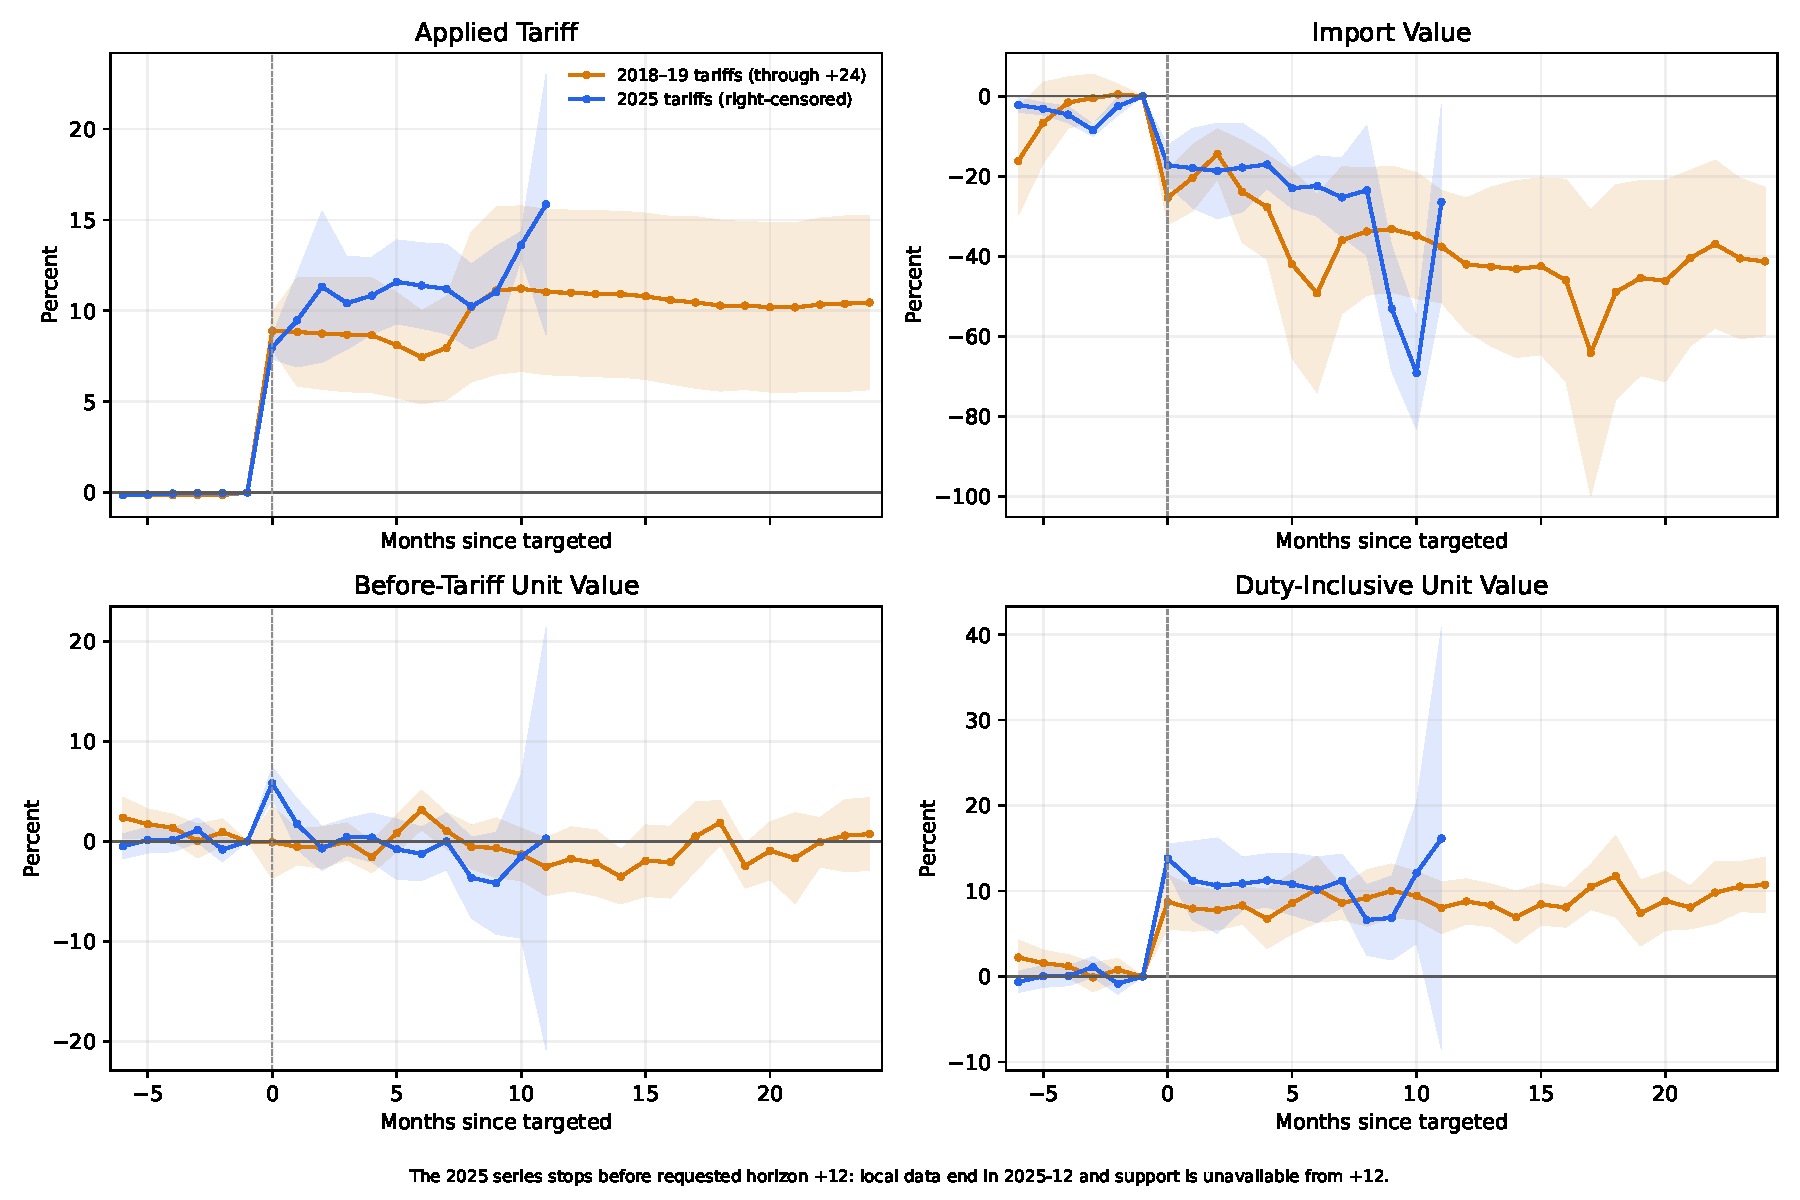
\includegraphics[width=0.96\textwidth]{../../figs/extension_2025/fk2025_figure4a_extended.pdf}
\caption{Import responses under the harmonized Fajgelbaum--Khandelwal
local-projection design. The 2018--19 treatment cohorts are followed through
$+24$ months using outcomes through December 2021. The 2025 axis is registered
through $+12$, but the line stops at $+11$: with local outcomes ending in
December 2025, the $+12$ risk set contains no treated observations. No
unsupported endpoint or 2026 outcome is imputed.}\end{figure}}{}

\IfFileExists{../../figs/extension_2025/fk2025_figure4b.pdf}{%
\begin{figure}[ht]\centering
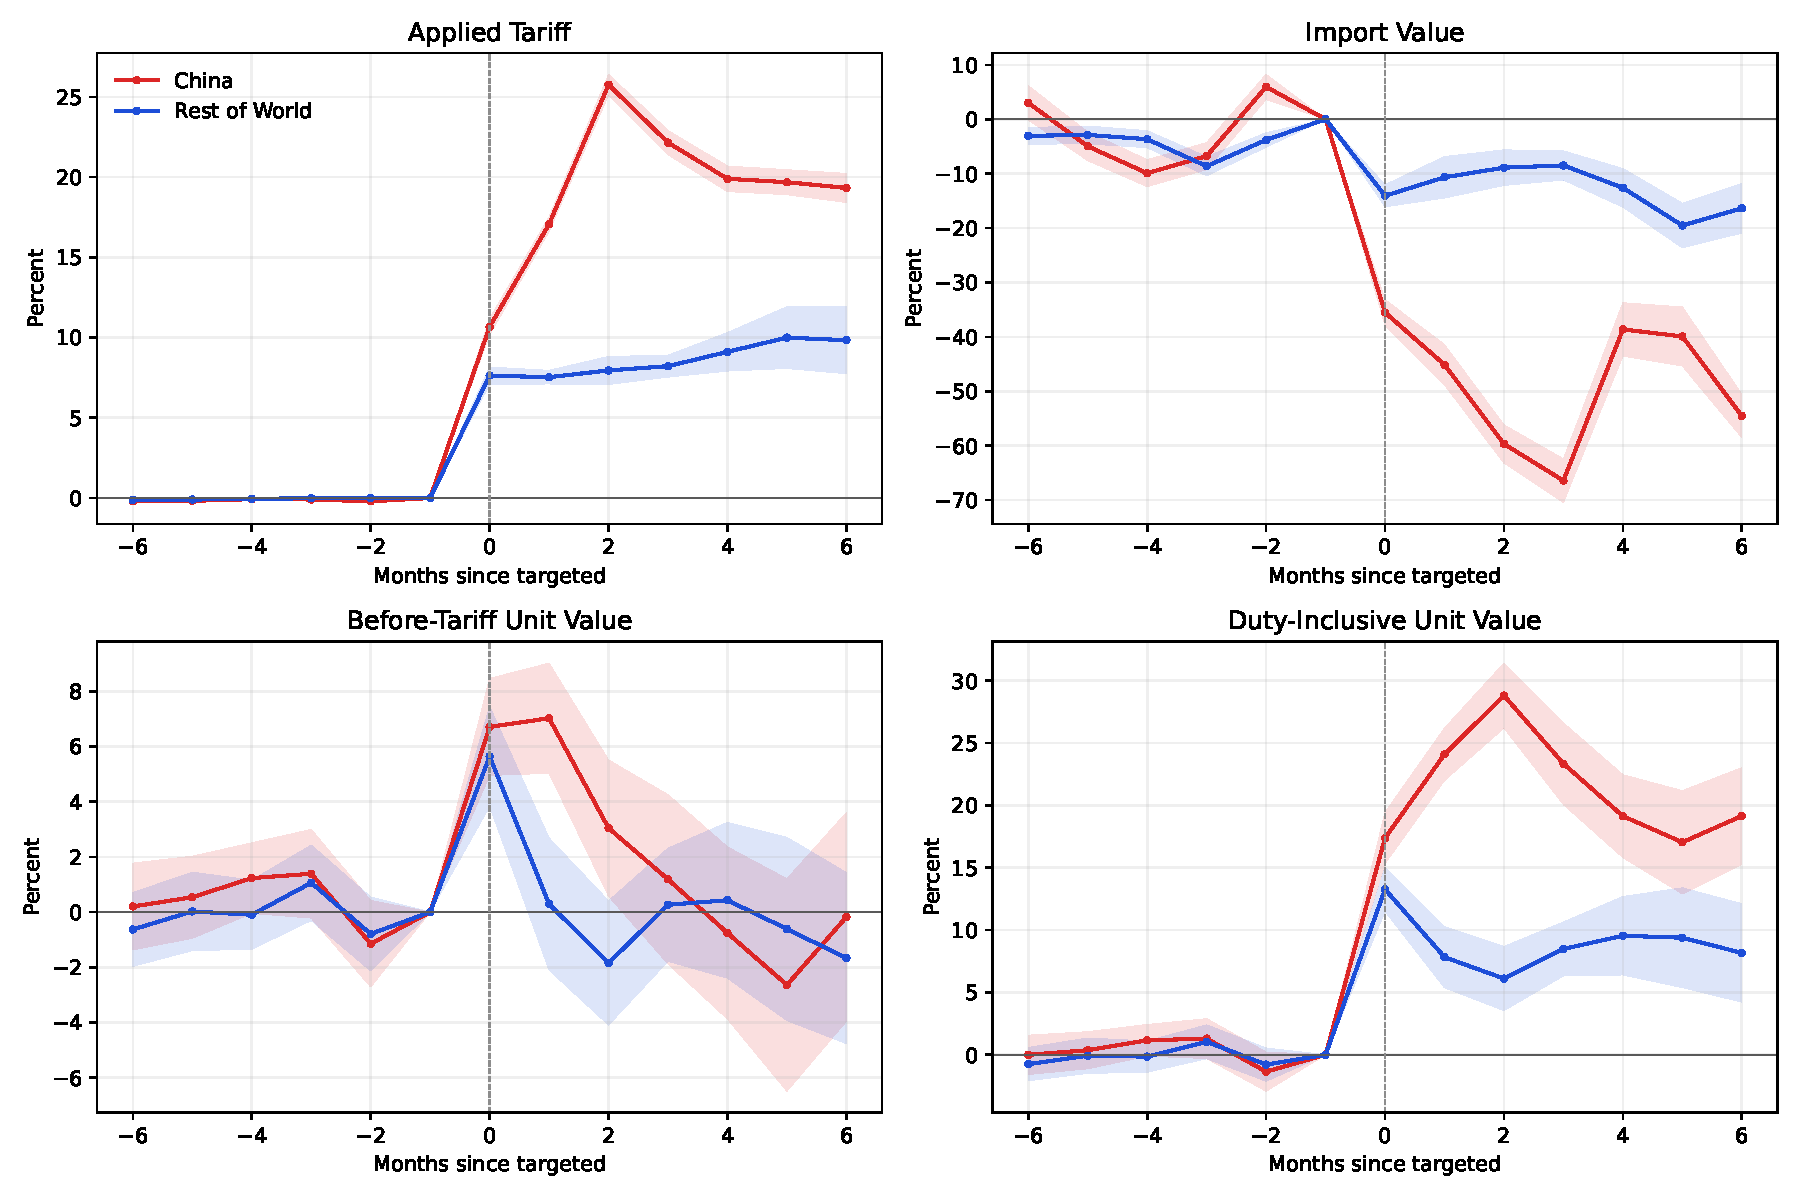
\includegraphics[width=0.96\textwidth]{../../figs/extension_2025/fk2025_figure4b.pdf}
\caption{Applied-tariff event studies for China and the rest of the world in
2025.}\end{figure}}{}

\subsection{Monthly cumulative local-projection pass-through}

The binary-treatment event study estimates cumulative outcome responses, not
pass-through elasticities. We therefore estimate a continuous cumulative
local-projection IV on the monthly origin--HS10 panel for each horizon
$h\geq0$, where $h$ is measured in months:
\begin{equation}
100\left[\log p^{duty}_{ig,t+h}-\log p^{duty}_{ig,t-1}\right]
=\alpha_{gt,h}+\alpha_{i,h}
+\beta_h\,100\left[
\log(1+\tau^{applied}_{ig,t+h})
-\log(1+\tau^{applied}_{ig,t-1})\right]
+\varepsilon_{ig,t,h}.
\label{eq:cumulative-lp-iv}
\end{equation}
The cumulative applied-tariff change is instrumented with the same endpoint
change in the independently constructed statutory tariff. The fixed effects
are HS10--base-month and origin; standard errors are clustered by origin and
HS8. Thus $\beta_h$ measures the cumulative change in duty-inclusive unit
value per cumulative change in the tariff actually paid. Complete
pass-through corresponds to $\beta_h=1$.

We absorb the two high-dimensional fixed effects by alternating projections
after recursively removing singleton groups. We then compute the scalar,
exactly identified 2SLS coefficient from the residualized outcome, applied
tariff, and statutory instrument. Inference uses the two-way CRV1 score
covariance (origin plus HS8 minus their intersection) and a $t$ critical
value based on the smaller cluster count. A synthetic equivalence test
requires numerical agreement of point estimates and clustered standard
errors within two percent of the formula-based reference implementation.

Every horizon uses a common sample with positive pre-duty and duty-inclusive
unit values at both endpoints. Since the Census definitions imply
\begin{equation}
\log p^{duty}_{igt}
=\log p_{igt}+\log(1+\tau^{applied}_{igt}),
\end{equation}
the corresponding pre-duty coefficient satisfies
$\widehat\beta^p_h=\widehat\beta^{duty}_h-1$ and has the same standard error.
We estimate equation~\eqref{eq:cumulative-lp-iv} directly and reject a
checkpoint unless the row-level identity holds to $10^{-8}$.

For the 2018 episode, base months are January 2018--December 2019 and outcomes
are followed through $h=24$. The independent paper-compatible statutory
ledger ends in December 2019. We hold each origin--HS10's last nonmissing
December-2019 rate fixed at later endpoints; an unmapped rate remains missing.
For 2025, base months are January--December 2025 and the instrument is the
independently constructed, calendar-day-weighted
\texttt{statutory\_paper\_coverage\_rate}. Outcomes observed through December
2025 support $h=0,\ldots,11$; no $h=12$ coefficient is imputed.

The historical duty-inclusive coefficient is 0.940 (SE 0.096) on impact,
1.090 (0.057) at six months, 1.201 (0.057) at twelve months, and 1.088
(0.052) at twenty-four months. Its first-stage $F$ statistic is never below
125.0. The results therefore indicate approximately complete cumulative
pass-through, with a modest temporary overshoot at intermediate horizons.

For 2025, duty-inclusive pass-through is 1.072 (SE 0.063) on impact, 1.037
(0.085) at three months, 1.018 (0.104) at six months, and 1.113 (0.182) at
eight months. It falls to 0.637 at month nine and to 0.365 at month eleven.
The late observations are much less precise and use a changing risk set:
effective observations fall from 1,465,779 at $h=0$ to 101,343 at $h=11$.
The $h=11$ 95-percent interval is $[-0.340,1.069]$, and the first-stage
$F$ remains 18.8. We therefore interpret the estimates through month eight
as evidence of near-complete pass-through and the later decline as
right-tail evidence with limited support, not as a precisely measured tariff
reversal.

\IfFileExists{../../figs/extension_2025/cumulative_pass_through_trade_war_2018.pdf}{%
\begin{figure}[ht]\centering
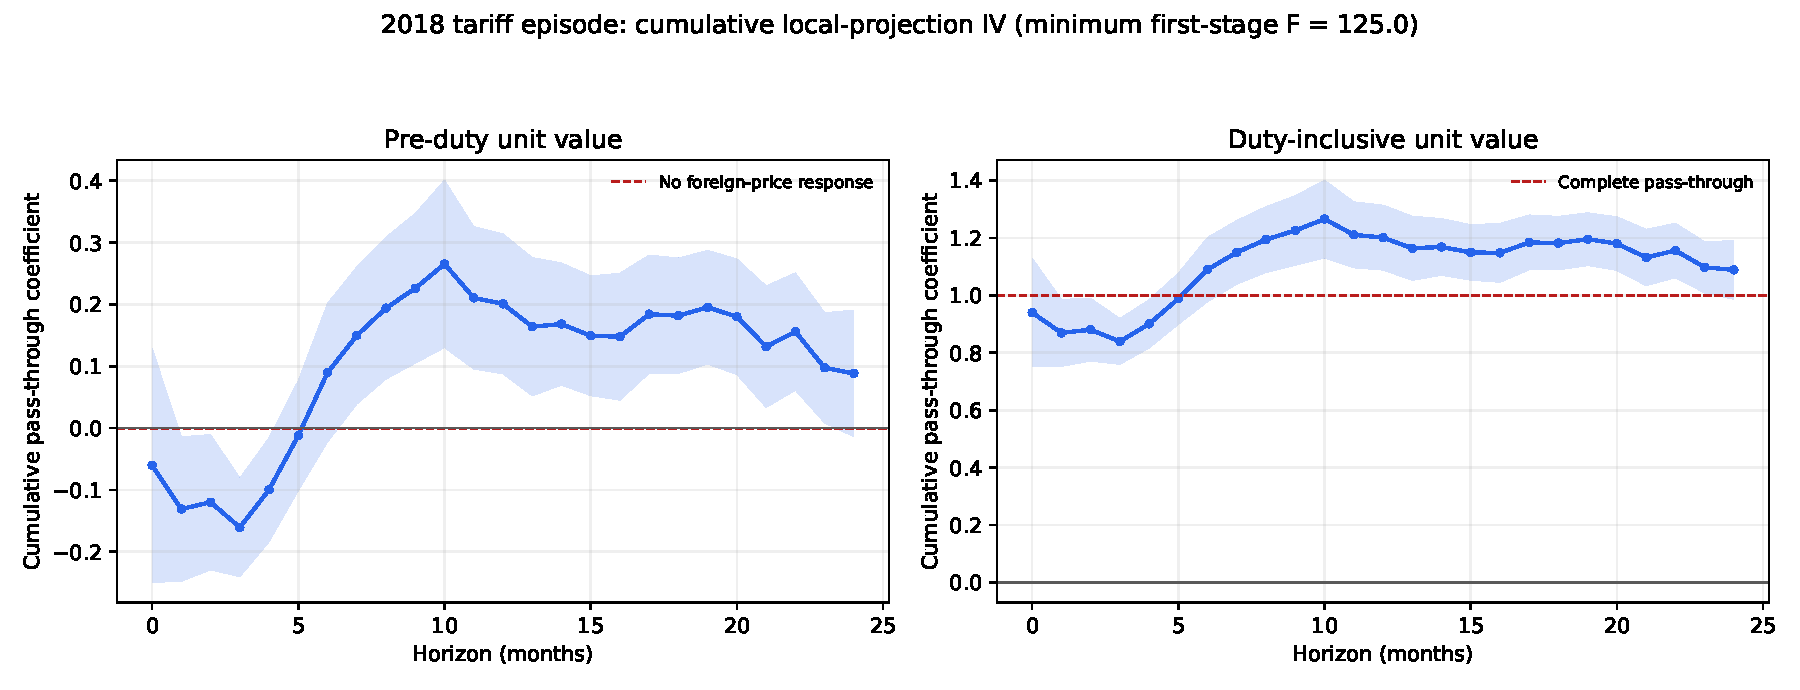
\includegraphics[width=0.96\textwidth]{../../figs/extension_2025/cumulative_pass_through_trade_war_2018.pdf}
\caption{Monthly cumulative local-projection IV pass-through for the 2018 tariff
episode. The left panel reports the pre-duty-price response; the right panel
reports duty-inclusive pass-through. Shaded regions are 95 percent confidence
intervals.}\label{fig:cumulative-lp-2018}
\end{figure}}{}

\IfFileExists{../../figs/extension_2025/cumulative_pass_through_tariffs_2025.pdf}{%
\begin{figure}[ht]\centering
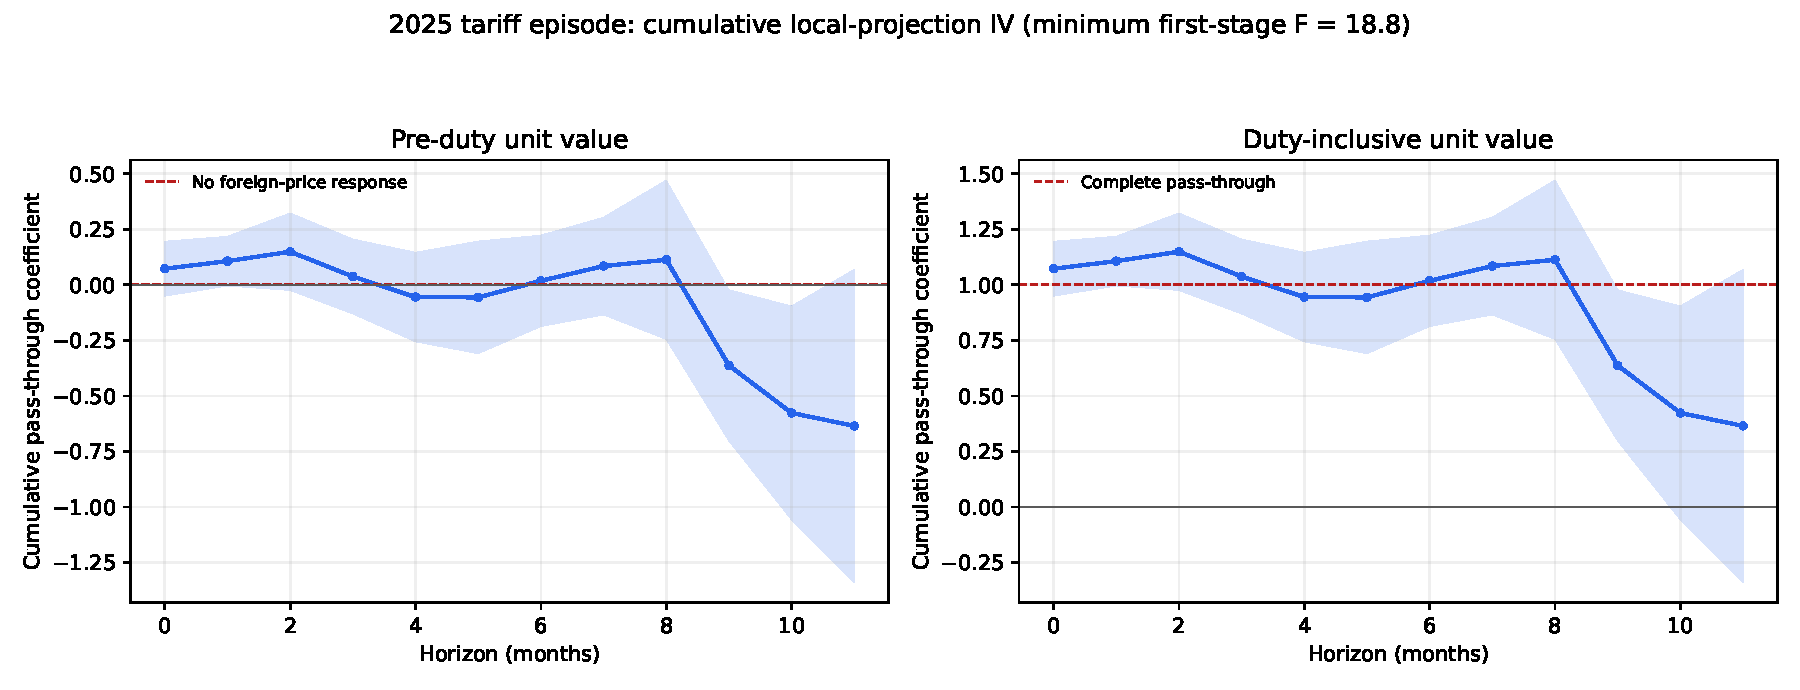
\includegraphics[width=0.96\textwidth]{../../figs/extension_2025/cumulative_pass_through_tariffs_2025.pdf}
\caption{Monthly cumulative local-projection IV pass-through for the 2025 tariff
episode. The last supported endpoint is $h=11$ because local outcomes end in
December 2025. Shaded regions are 95 percent confidence intervals.}
\label{fig:cumulative-lp-2025}
\end{figure}}{}

\subsection{Quarterly instrumental-variable estimates}

This is a separate benchmark from the monthly cumulative local projections
above. The preferred pass-through estimate collapses the data to
origin--HS10--quarter and estimates
\begin{equation}
\Delta\log y_{igt}
=\alpha_{gt}+\alpha_i+
\beta\Delta\log(1+\tau^{applied}_{igt})+\varepsilon_{igt},
\end{equation}
instrumenting the applied tariff with the independently reconstructed
statutory tariff.  Statutory rates are calendar-day weighted within month and
then consumption-value weighted within quarter.  The benchmark uses the
paper's January 2024--November 2025 cutoff; a separately labeled robustness
includes December.  Entry-dependent content, certification, in-transit, and
rate-provision ambiguities remain disclosed and are never silently replaced
with zero.

We use two explicit statutory instruments. The primary
\texttt{paper\_coverage} instrument retains all rows with a mapped ordinary
rate and applies every observable published partner--product schedule. It
omits unobservable entry-level components, while preserving ambiguity flags.
The \texttt{deterministic} sensitivity retains only simple ad-valorem ordinary
rates, observable flat partner schedules, no complex content or certification
scope, and no unverified inherited Section~201/232 component. Neither
instrument is filled with an authors-package tariff.

\begin{table}[ht]
\centering
\caption{Quarterly import pass-through: paper and independent replication}
\label{tab:fk2025-table4}
\begin{tabular}{lrr}
\toprule
Outcome & Paper estimate (SE) & Replication estimate (SE)\\
\midrule
First stage & 0.42 (0.06) & 0.376 (0.052)\\
Import value & -1.81 (0.50) & -1.922 (0.552)\\
Quantity & -1.71 (0.54) & -1.888 (0.622)\\
Pre-duty unit value & -0.10 (0.06) & -0.033 (0.080)\\
Duty-inclusive unit value & 0.90 (0.06) & 0.967 (0.080)\\
\bottomrule
\end{tabular}
\end{table}

The paper-cutoff replication contains 1,224,214 observations, compared with
1,192,687 in the paper, and has a first-stage $F$-statistic of 51.51, compared
with 52.4. The first stage, value, and quantity estimates are within one
reported paper standard error. The two price estimates are 0.0668 from the
reported values, narrowly outside the registered 0.0600 tolerance. Their
accounting identity holds exactly:
\begin{equation}
\widehat\beta_{p^{duty}}-\widehat\beta_p=1.
\end{equation}
Accordingly, the preregistered paper-cutoff Table~4 gate is recorded as a
narrow failure. The complete-December robustness produces -0.044 for
pre-duty price and 0.956 for duty-inclusive price and passes all registered
Table~4 checks. The strict deterministic sensitivity contains only 369,936
observations and is not treated as the paper-comparable baseline.

Monthly, quarterly, and semiannual robustness estimates use period-over-period
changes. The annual specification follows Table A.3 by taking year-over-year
changes in quarterly observations, such as 2025Q1 relative to 2024Q1.
The semiannual pre-duty-price estimate is -0.155, nearly identical to the
paper's -0.15. The annual estimate is -0.014 with $F=18.42$ and 669,849
observations, materially different from the paper's -0.08, $F=1421.4$, and
532,390 observations. This annual discrepancy remains unresolved and is not
classified as a replicated robustness result.
